\documentclass[12pt]{article}
\usepackage[a5paper, margin=0.5cm]{geometry}

\usepackage[default]{comfortaa}
\usepackage[T1]{fontenc}


\usepackage[dvipsnames]{xcolor}
\usepackage{pgfplots}
\usepackage{pgfplotstable}
\usepackage{tikz}
\usetikzlibrary{calc}
\usetikzlibrary{positioning,shapes,arrows, fit, shapes.geometric}

\pgfplotsset{compat=1.8}

\makeatletter
\pgfplotsset{
	/pgfplots/flexible xticklabels from table/.code n args={3}{%
		\pgfplotstableread[#3]{#1}\coordinate@table
		\pgfplotstablegetcolumn{#2}\of{\coordinate@table}\to\pgfplots@xticklabels
		\let\pgfplots@xticklabel=\pgfplots@user@ticklabel@list@x
	}
}
\makeatother

\definecolor{ggreen}{HTML}{50CD50}


\usepackage{graphicx}
\usetikzlibrary{positioning,arrows,shapes,fit,  shapes.geometric}



\pgfplotstableread[header=has colnames,
columns/TestSet/.style={string type},
]{%
TestSet	{Most Commonly Mentioned}	{ML Classical Feats.}	{ML Word Emb.}
ASOIAF	0.9140625	0.9765625	0.97265625
SOC	0.791208791	0.934065934	0.945054945
WOT	0.659722222	0.736111111	0.680555556
}{\res}

\renewcommand{\familydefault}{\sfdefault}


\begin{document}
\centering
\thispagestyle{empty}
\null
\vspace{-0.3cm}
{\Huge NovelPerpective\\}
{\Large Identifying Point of View Characters\\}
\vspace{0.4cm}
%\hspace{-0.1cm}
\begin{tikzpicture}
\begin{axis}[ybar,
	xticklabels from table={\res}{TestSet},
	legend style={at={(0.5,-0.5)}, anchor=north,legend columns=-1, draw=none},
%	enlargelimits=0.3,
	ymin = 0, ymax=1,
	enlarge x limits=0.2,
	xticklabel style={text width=8em, align=center},
	xtick = data,
	width=0.7\textwidth, height= 3.5cm,
	bar width=0.6cm,
	yticklabel={$\mathsf{\pgfmathparse{\tick*100}\pgfmathprintnumber{\pgfmathresult}}$\small\%},
	ytick = {0, 0.25, 0.50, 0.75, 1.00},
	ylabel = Accuracy,
	axis line style={draw=none},
	x tick style={draw=none},
	ytick pos=left,
]
%\addplot[style={bblue,fill=bblue,mark=none}] table[x expr=\coordindex, y={ML Word Emb.}] {\res};
\addplot[style={top color=Cyan, bottom color=Blue, draw=none, mark=none}] table[x expr=\coordindex, y={ML Word Emb.}] {\res};
\addplot[style={top color=Orange, bottom color=Brown, draw=none, mark=none}] table[x expr=\coordindex, y={ML Classical Feats.}] {\res};
\addplot[style={top color=Gray, bottom color=Purple, draw=none, mark=none}] table[x expr=\coordindex, y={Most Commonly Mentioned}] {\res};
\legend{{Word Emb.},{Classical Feats.},{Baseline}}
\end{axis}
\end{tikzpicture}

\vspace{0.1cm}
{\large Core idea: Train a binary classifier to determine if a name token is that of the POV character, based on a feature vector representing that token's usage.\\
	 Use this as a POV-likelihood score for that named entity.}
\vspace{0.1cm}

\resizebox{\textwidth}{!}{
	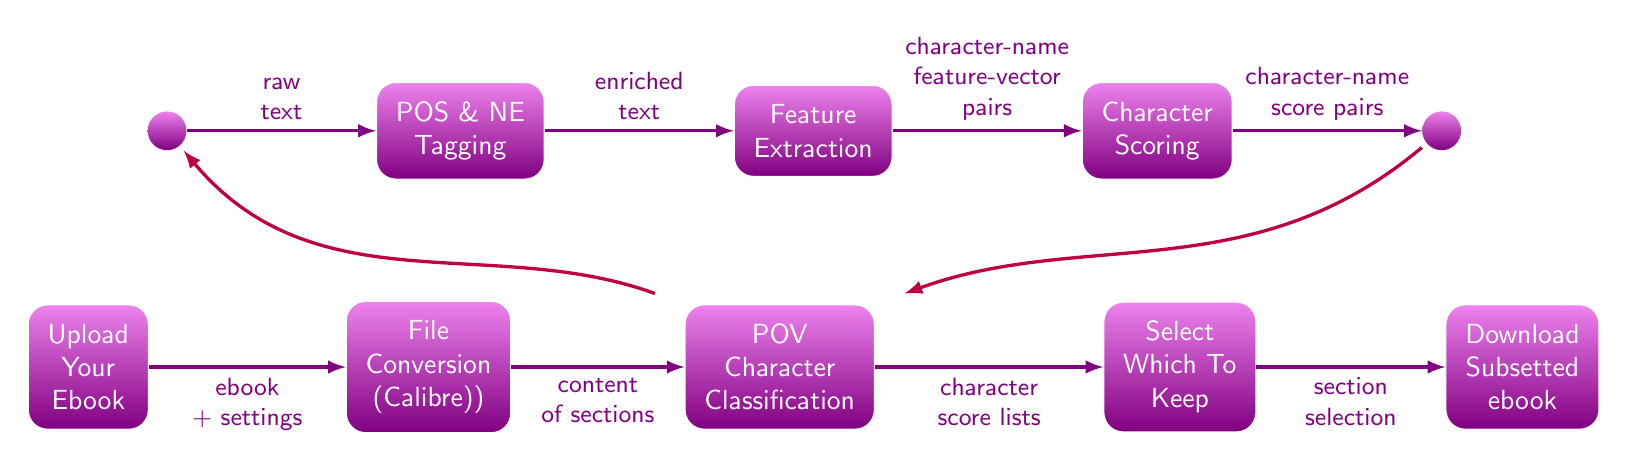
\begin{tikzpicture}[
		>=latex,
		every text node part/.style={align=center},
		auto,
		node distance=2.4, 
		->,
		every edge/.append style={very thick, Purple, every node/.style={font=\small}},
		every node/.style={rounded corners=7pt, fancy, inner sep=7pt},
		gather/.style = { very thick, purple, shorten <= 0.4cm},
		fancy/.style= {draw=none, shade, 
			color=White,
			top color=Violet, bottom color=Purple
		}
	]	
	\begin{scope}[yshift=3cm]		
		\node(start1){};
		\node(enrich)[draw, right=of start1] {POS \& NE \\ Tagging};
		\node(features)[draw, right=of enrich] {Feature\\ Extraction};
		\node(scoring)[draw, right=of features] {Character\\Scoring};				
		\node(end)[right=of scoring] {};
		
		\path (start1) edge node[]{raw\\ text}  (enrich);
		\path (enrich) edge node[above]{enriched\\text} (features);
		\path (features) edge node[above]{character-name\\feature-vector\\pairs
		} (scoring);
		\path (scoring) edge node[above]{character-name\\score pairs
		} (end);
	\end{scope}
	
	\begin{scope}[xshift=-1cm]		
		\node(start)[draw] {Upload\\ Your \\Ebook};
		\node(convert)[draw, right=of start, xshift=0.1cm] {File\\Conversion\\(Calibre))};
		\node(classify)[draw, right=of convert, xshift=-0.2cm] {POV\\Character\\Classification};
		\node(select)[draw, right= of classify, xshift=0.5cm] {Select\\ Which To \\ Keep};
		\node(download)[draw, right=of select] {Download \\ Subsetted \\ ebook};
		
		\path (start) edge[below] node[below]{ebook \\ + settings}  (convert);
		\path (convert) edge[below] node[below]{content\\ of sections} (classify);
		\path (classify) edge[below] node[below]{character\\score lists} (select);
		\path (select) edge[below] node[below]{section\\selection} (download);	
		
		\draw[->, gather] (classify.north west) to[out=160, in=-50] (start1);
		\draw[<-, gather] (classify.north east) to[out=20, in=-140] (end);
	\end{scope}
	
	\end{tikzpicture}
}

\vspace{0.1cm}
{\Large Skip the chapters about the boring characters.}
{\Large Read a character's story without interruptions.}
{\LARGE {http://novelperspective.ucc.asn.au/}
\vspace{0.1cm}

\begin{tikzpicture}
\node[draw, text width=0.9\textwidth, %text height=3cm,
ultra  thick, rounded corners=7pt,
White, fill=Blue,
](frame){
\normalsize
Lyndon White, PhD Candidate \\
The University of Western Australia\\
\vspace{0.1cm}
{lyndon.white@ucc.gu.uwa.edu.au}\\
{https://white.ucc.asn.au}\\
\vspace{0.2cm}
Talk to me about NLP, ML and Data Science\newline in JuliaLang
\hfill
\includegraphics[width=1em]{ghlogos/juliaeditorsupport}
\includegraphics[width=1em]{ghlogos/juliatext}
\includegraphics[width=1em]{ghlogos/juliastring}
\includegraphics[width=1em]{ghlogos/juliaml}
\includegraphics[width=1em]{ghlogos/juliacollections}
\includegraphics[width=1em]{ghlogos/juliadiffeq}
\includegraphics[width=1em]{ghlogos/juliagraphics}
\includegraphics[width=1em]{ghlogos/ucc}
\hspace{3cm}\null
\\
};


\begin{scope}[xshift=5.1cm]
\def\bord{4pt}
\def\ig{\includegraphics[height=3.3cm,keepaspectratio]{portrait}}
\node [inner sep=0pt](mypicture) at (0,0) {\phantom{\ig}};
\clip[rounded corners=5mm] ($(mypicture.south west)+(\bord,\bord)$) rectangle ($(mypicture.north east)-(\bord,\bord)$);
\node[inner sep=0pt, xscale=-1](mypicture) at (0,0) {\ig};
\end{scope}


\end{tikzpicture}





\end{document}